% ============================================================
\chapter{Interpolation Polynomiale}
\label{ch:interpolation}
% ============================================================

\section{Exemple motivant}
On dispose de mesures de temp\'erature \`a 5 instants. On veut estimer la temp\'erature \`a un instant interm\'ediaire. L'interpolation polynomiale construit un polyn\^ome passant exactement par les points mesur\'es.

\section{Probl\`eme d'interpolation}

\begin{theoreme}[Existence et unicit\'e]
\'Etant donn\'es $n+1$ points distincts $(x_0,y_0),\ldots,(x_n,y_n)$, il existe un \textbf{unique} polyn\^ome $p_n\in\mathcal{P}_n$ tel que $p_n(x_i)=y_i$ pour tout $i$.
\end{theoreme}

\begin{proof}
La matrice de Vandermonde $V_{ij}=x_i^j$ est inversible car $\det(V)=\prod_{i>j}(x_i-x_j)\neq 0$.
\end{proof}

\section{Forme de Lagrange}\index{Lagrange}

\begin{definition}
\[
p_n(x) = \sum_{i=0}^n y_i\,L_i(x), \quad L_i(x)=\prod_{\substack{j=0\\j\neq i}}^n\frac{x-x_j}{x_i-x_j}.
\]
Les $L_i$ sont les \textbf{polyn\^omes de base de Lagrange} : $L_i(x_j)=\delta_{ij}$.
\end{definition}

\section{Forme de Newton}\index{Newton!interpolation}

\begin{definition}[Diff\'erences divis\'ees]
\[
f[x_i]=f(x_i), \quad f[x_i,\ldots,x_{i+k}]=\frac{f[x_{i+1},\ldots,x_{i+k}]-f[x_i,\ldots,x_{i+k-1}]}{x_{i+k}-x_i}.
\]
\end{definition}

\begin{definition}[Forme de Newton]
\[
p_n(x) = f[x_0]+f[x_0,x_1](x-x_0)+\cdots+f[x_0,\ldots,x_n]\prod_{j=0}^{n-1}(x-x_j).
\]
\'Evaluation par l'algorithme de Horner g\'en\'eralis\'e : $\BigO(n)$ op\'erations.
\end{definition}

\section{Erreur d'interpolation}

\begin{theoreme}[Erreur d'interpolation]\label{thm:erreur-interp}
Si $f\in C^{n+1}([a,b])$, alors pour tout $x\in[a,b]$ :
\[
f(x)-p_n(x) = \frac{f^{(n+1)}(\xi_x)}{(n+1)!}\prod_{i=0}^n(x-x_i),
\]
o\`u $\xi_x\in(a,b)$ d\'epend de $x$.
\end{theoreme}

\begin{proof}
Posons $w(t)=\prod(t-x_i)$ et $\varphi(t)=f(t)-p_n(t)-\lambda w(t)$ avec $\lambda$ choisi pour que $\varphi(x)=0$ (pour un $x$ fix\'e $\neq x_i$). Alors $\varphi$ s'annule en $n+2$ points. Par Rolle appliqu\'e $n+1$ fois, $\varphi^{(n+1)}$ s'annule en un point $\xi$. Or $\varphi^{(n+1)}=f^{(n+1)}-\lambda(n+1)!$, d'o\`u $\lambda=f^{(n+1)}(\xi)/(n+1)!$.
\end{proof}

\begin{attention}
Le \textbf{ph\'enom\`ene de Runge} : pour $f(x)=1/(1+25x^2)$ sur $[-1,1]$ avec des n\oe uds \'equidistants, l'erreur d'interpolation \emph{diverge} quand $n\to\infty$ pr\`es des bords.
\end{attention}

\begin{center}
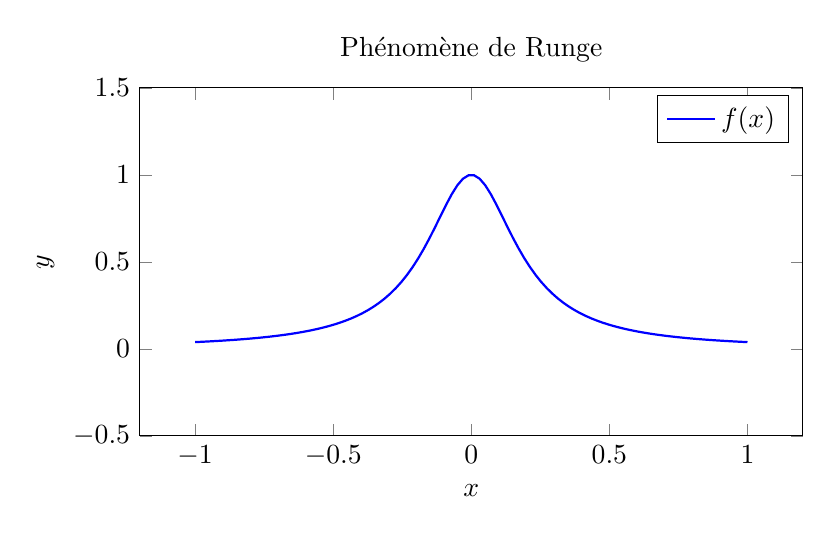
\begin{tikzpicture}
\begin{axis}[
  width=10cm, height=6cm, domain=-1:1, samples=100,
  xlabel=$x$, ylabel=$y$, ymin=-0.5, ymax=1.5,
  title={Ph\'enom\`ene de Runge}
]
\addplot[thick,blue] {1/(1+25*x^2)};
\addlegendentry{$f(x)$}
\end{axis}
\end{tikzpicture}
\end{center}

\section{N\oe uds de Tchebychev}\index{Tchebychev!noeuds}

\begin{definition}
Les n\oe uds de Tchebychev sur $[-1,1]$ :
\[
x_k = \cos\left(\frac{2k+1}{2(n+1)}\pi\right), \quad k=0,\ldots,n.
\]
Ils minimisent $\max_{x\in[-1,1]}|\prod(x-x_i)|$.
\end{definition}

\begin{theoreme}
Avec les n\oe uds de Tchebychev : $\max|w(x)|\leq 2^{-n}$, ce qui \'evite le ph\'enom\`ene de Runge pour les fonctions analytiques.
\end{theoreme}

\section{Splines cubiques}\index{spline}

\begin{definition}[Spline cubique d'interpolation]
$s\in C^2([a,b])$, $s|_{[x_i,x_{i+1}]}\in\mathcal{P}_3$, $s(x_i)=y_i$. Conditions aux bords :
\begin{itemize}
\item \textbf{Naturelle} : $s''(x_0)=s''(x_n)=0$.
\item \textbf{Clamp\'ee} : $s'(x_0)=f'(x_0)$, $s'(x_n)=f'(x_n)$.
\end{itemize}
\end{definition}

\begin{theoreme}[Erreur spline cubique]
Si $f\in C^4$ et $h=\max(x_{i+1}-x_i)$ :
\[
\|f-s\|_\infty \leq \frac{5}{384}h^4\|f^{(4)}\|_\infty.
\]
\end{theoreme}

\section{Impl\'ementation}

\begin{codeblock}[title=\textbf{Python}]
\begin{minted}{python}
import numpy as np
from scipy.interpolate import lagrange, CubicSpline
import matplotlib.pyplot as plt

# Interpolation de Lagrange
x_nodes = np.array([-1, -0.5, 0, 0.5, 1])
f = lambda x: 1 / (1 + 25*x**2)
y_nodes = f(x_nodes)
p = lagrange(x_nodes, y_nodes)

x_fine = np.linspace(-1, 1, 300)
plt.figure(figsize=(10, 5))
plt.plot(x_fine, f(x_fine), 'b-', label='f(x)', lw=2)
plt.plot(x_fine, p(x_fine), 'r--', label=f'Lagrange deg {len(x_nodes)-1}')
plt.plot(x_nodes, y_nodes, 'ko', markersize=8)
plt.legend(); plt.title("Interpolation de Lagrange")
plt.savefig("ch05_lagrange.pdf"); plt.show()

# Noeuds de Tchebychev
n = 15
cheb = np.cos((2*np.arange(n+1)+1)/(2*(n+1))*np.pi)
y_cheb = f(cheb)
p_cheb = lagrange(cheb, y_cheb)
print(f"Erreur equidist (n=15): {np.max(np.abs(f(x_fine)-lagrange(np.linspace(-1,1,16), f(np.linspace(-1,1,16)))(x_fine))):.4f}")
print(f"Erreur Tchebychev (n=15): {np.max(np.abs(f(x_fine)-p_cheb(x_fine))):.6f}")

# Spline cubique
cs = CubicSpline(x_nodes, y_nodes)
print(f"Spline en 0.25: {cs(0.25):.6f}, exact: {f(0.25):.6f}")
\end{minted}
\end{codeblock}

\begin{codeblock}[title=\textbf{Julia}]
\begin{minted}{julia}
using Interpolations

f(x) = 1 / (1 + 25x^2)
nodes = [-1.0, -0.5, 0, 0.5, 1.0]
vals = f.(nodes)

# Differences divisees (Newton)
function divided_diff(x, y)
    n = length(x)
    F = copy(y)
    for j in 2:n, i in n:-1:j
        F[i] = (F[i] - F[i-1]) / (x[i] - x[i-j+1])
    end
    return F
end
println("Coefs Newton: ", divided_diff(nodes, vals))
\end{minted}
\end{codeblock}

\section{Exercices}

\begin{exercice}[$\star$]
Construire le polyn\^ome de Lagrange passant par $(0,1)$, $(1,3)$, $(2,7)$ et v\'erifier.
\end{exercice}

\begin{exercice}[$\star\star$]
D\'emontrer le th\'eor\`eme~\ref{thm:erreur-interp} en d\'etail.
\end{exercice}

\begin{exercice}[$\star\star$]
Comparer l'erreur d'interpolation avec n\oe uds \'equidistants vs.\ Tchebychev pour $f(x)=1/(1+25x^2)$, $n=5,10,15,20$.
\end{exercice}

\begin{exercice}[$\star\star\star$ -- Projet]
Impl\'ementer l'interpolation de Hermite (donn\'ees de $f$ et $f'$). Appliquer \`a la construction de courbes de B\'ezier.
\end{exercice}

\begin{formules}
\begin{align*}
L_i(x) &= \prod_{j\neq i}\frac{x-x_j}{x_i-x_j} \\
f(x)-p_n(x) &= \frac{f^{(n+1)}(\xi)}{(n+1)!}\prod(x-x_i) \\
x_k^{\text{Tcheb}} &= \cos\!\left(\frac{2k+1}{2(n+1)}\pi\right) \\
\|f-s\|_\infty &\leq \frac{5}{384}h^4\|f^{(4)}\|_\infty
\end{align*}
\end{formules}
